\documentclass[french,12pt]{article}
\usepackage{babel}

\usepackage[utf8]{inputenc}%encodage des caractères
\usepackage[T1]{fontenc}%encodage de la police
\usepackage{graphicx}
\usepackage{amsmath}
\usepackage{hyperref}
\usepackage{tikz}
\usepackage{listings}
\usepackage[linesnumbered,ruled,french,onelanguage]{algorithm2e} 
\setlength{\parindent}{0pt} 

\title{Rapport Méthode de Conception}
\author{Antonin Montagne, Lou-Anne Gautherie, Nathan Sakkriou, \\
Yanis Habarek}
\date{25 Novembre 2022}

\begin{document}

\maketitle

\begin{figure}[h]
	\begin{center}
		
\includegraphics[scale=0.4]{img/fond.png}	
	\end{center}
\end{figure}

\begin{figure}[b]
	\begin{center}
		
\includegraphics[scale=0.7]{img/unicaen.png}	
	\end{center}
\end{figure}

\thispagestyle{empty}
\setcounter{page}{0}
\newpage

\tableofcontents
\newpage

\section{Introduction}

\subsection{Plan du rapport}

Nous évoquerons d'abord quels étaient nos objectifs de départ (\ref{objectifs}), puis nous détaillerons les différentes étapes de la création de notre projet avec les rôles de chacuns (\ref{organisation}). Ensuite nous présenterons l'architecture de ce projet (\ref{architecture}), ainsi que les éléments techniques utilisées (\ref{elemtech}) dans notre code. Finalement nous terminerons par une courte conclusion (\ref{conclusion}).

\subsection{Objectifs du projet} \label{objectifs}

Nous avions pour but de créer un jeu de Blackjack. Certaines contraintes nous étaient données :
\begin{itemize}
	\item Respecter la forme MVC.
	\item Créer une dépendance entre une librairie "\texttt{cartes}" et un jeu "\texttt{blackjack}".	
\end{itemize}

\section{Fonctionnalités implémentées} \label{organisation}

\subsection{Description des fonctionnalités}

A partir de l'accueil, il est d'abord possible de vérifier les règles du blackjack en cliquant sur le bouton "\textsc{règles du jeu}". \\
Le clic du bouton renverra le joueur sur le site \textit{guide-blackjack.com/regles-du-black-jack.html}, qui contient les règles de ce jeu. \\\\
Il est aussi proposé de lancer une partie à l'aide du bouton "\textsc{nouvelle partie}". \\
Le clic du bouton ouvrira un formulaire qui demandera à l'utilisateur, combien de joueur veut-il rentrer pour cette partie ainsi que le style de cartes qu'il souhaitera. Une fois le nombre de joueur rentré, le jeu se lancera après avoir cliqué sur "\textsc{Commencer}". Le joueur commencera la partie, il peut soit tirer une carte, soit ne rien faire (boutons  "\textsc{Hit}" et "\textsc{Stop}"). Si il choisit de ne rien faire, le tour passe au croupier. Le plus proche de 21 sans dépasser gagne la partie. Une fois la partie terminée, une fenêtre pop-up avec le nom de celui qui a gagné et un bouton "\textsc{OK}" qui renverra le joueur sur la page d'accueil.\\\\
Depuis l'accueil, il est finalement possible de fermer la fenêtre en appuyant sur "\textsc{Cliquer}". 

\subsection{Organisation du projet}

Pour commencer, Nathan a codé toute la librairie \textsl{cartes.jar}. \\
Il a d'abord définit ce qui est une carte dans la classe \textsf{Card}. Une carte est définit par une \texttt{value} et une \texttt{color}. Chaque carte est également définit par une image qui est récupérée par la \texttt{getImgPath}. Il y a deux styles différents de cartes: \textit{classique} et \textit{vintage}. Il a codé plusieurs fonctions de comparaisons comme la fonction \texttt{compareTo} qui compare les valeurs d'objets, et la fonction \texttt{equals} qui vérifie si deux objets sont égaux.\\\\
Ensuite il a codé la classe \textsl{Deck} qui définit un paquet de cartes. Un deck est représenté par une \texttt{ArrayList<Card>}. Cette classe contient une fonction \texttt{shuffleDeck} pour mélanger les cartes du deck, deux fonctions \texttt{addCardToEnd} et \texttt{addCardToHead} qui permettent respectivement d'ajouter une carte à la fin ou au début du paquet. Il y a également un fonction \texttt{drawCard} qui représente une carte piochée; elle est enlevée du deck et retourne la carte piochée.\\\\
Ensuite il a codé une main dans la classe \textsl{Hand}; une main est définit par une \texttt{ArrayList<Card>} et un \texttt{Deck}. Elle possède des fonctions pour: 
\begin{itemize}
	\item tirer une carte de la main (\texttt{getCard}), 
	\item retourner les cartes de la main afin de voir leurs valeurs ou non
		  (\texttt{changeShowHand}),
	\item ajouter ou retirer une carte de la main (\texttt{addCard} et
		  \texttt{removeCard}),
	\item réinitialiser la main (\texttt{resetHand}),
	\item jouer une carte (\texttt{playCard}),
	\item et une dernière fonction de comparaison (\texttt{compareTo})\\
\end{itemize}
Finalement il a créer une classe \textsl{DeckFactory}, qui génère des \textsl{Deck} prédéfinis. Elle contient deux fonctions qui initialisent des deck:
\begin{enumerate}
	\item \texttt{get52DeckCard}; un deck de 52 cartes (as à roi),
	\item \texttt{get40DeckCard}; un deck de 40 cartes (as à 10).\\
\end{enumerate}
Dans le package \textsl{Blackjack} se trouve la classe \textsl{Party} codée par Nathan. Cette classe représente simplement une partie de Blackjack. Les éléments de cette classe sont:
\begin{itemize}
	\item un \texttt{Deck deck} qui est le jeu de cartes,
	\item une \texttt{ArrayList<Hand> listHand} qui est la liste de toutes
		  les mains de tous les joueurs,
	\item une \texttt{ArrayList<Integer> listSumHand} qui est la liste des
		  sommes des mains de tous les joueurs,
	\item une \texttt{Hand dealerHand} qui est la main du dealer,
	\item un \texttt{Integer sumDealerHand} qui est la somme de la main du
		  dealer,
	\item un \texttt{Integer NB$\_$CARD$\_$INITIAL$\_$DRAW} qui est le
		  nombre de cartes initial d'une main au début de partie
		  (initialisé ici à 2),
	\item un \texttt{Integer AS$\_$VALUE} qui est la valeur que l'as peut
		  prendre (soit 1, soit 11),
	\item et un \texttt{HashMap<String, Integer> 
		  RELATION$\_$NUMBER$\_$VALUE} qui est un dictionnaire contenant
		  les relations entre les valeurs des cartes.\\
\end{itemize}
Plusieurs méthodes y sont définies:
\begin{itemize}
	\item \texttt{generateRELATION$\_$NUMBER$\_$VALUE}, génère dans la
		  \texttt{HashMap \\ RELATION$\_$NUMBER$\_$VALUE} la relation entre
		  les "values" d'une carte et leurs valeurs numériques au
		  blackjack.
	\item \texttt{addHand} ajoute une main dans la partie,
	\item \texttt{initialDraw} représente le tirage initial de 2 cartes par
		  personne et d'une carte pour le croupier,
	\item \texttt{getSumHandValue} permet d'insérer dans les attributs
		  correspondant la somme des mains des joueurs et du croupier,
	\item \texttt{getSumHandValueOfOneHand} permet d'obtenir la valeur de
		  la main donnée,
	\item \texttt{getSumDealerHand} calcule la somme des cartes du
		  croupier,
	\item \texttt{handChoice} définit le choix du joueur lorsque c'est son
		  tour (tirer une carte -> return true, ou ne rien faire -> return
		  false),
	\item \texttt{askChoiceConsole} demande au joueur le choix qu'il veut
		  faire (méthode valable uniquement en console), s'il veut tirer,
		  il doit tapper 1, s'il veut ne rien faire, il doit tapper 2.
	\item \texttt{allHandTurn} permet de faire jouer tous les utilisateurs
		  chacun leurs tour (méthode valable uniquement en console),
	\item \texttt{dealerTurn} permet de jouer le tour du dealer,
	\item \texttt{AIPlayerTurn} permet de définir la manière de jouer des
		  intelligences artificielles,
	\item \texttt{checkWhoWin} vérifie les conditions de victoire du
		  croupier et des joueurs; si la somme des cartes du croupier vaut
		  plus de 21, tous les autres joueurs gagnent, si un joueur est
		  plus près de 21 que les autres, il gagne, et si un joueur dépasse
		  21, il perd.
	\item \texttt{completeTurn} permet de jouer un tour complet; les
		  joueurs jouent, le croupier joue, et on vérifie qui a gagné à la
		  fin du tour.
	\item et \texttt{launchGame} permet de lancer une partie (méthode
		  valable uniquement en console); les cartes sont distribuées à
		  l'aide de la méthode \texttt{initialDraw}, les sommes des mains
		  sont obtenues grâce à \texttt{getSumHandValue} et
		  \texttt{getSumDealerHand}.\\
\end{itemize}

Passons maintenant à la vue, codée par Yannis, Antonin et Lou-Anne. En premier lieu, dans le package \textsl{View} se trouve la classe \textsl{BasicPage} codée par Yannis, qui est la fenêtre de base utilisée dans toutes les autres classes de \textsl{View}. Elle contient des balises HTML et du style CSS, mais aussi les images de fond durant tout le lancement du jeu. 3 images y sont définies:
\begin{enumerate}
	\item l'image de fond lors du lancement à l'aide de la méthode 
		  \texttt{setBackgroundLaunch},
	\item l'image de fond de la page d'accueil à l'aide de la méthode
		  \texttt{setBackgroundHome},
	\item et l'image de fond du jeu à l'aide de la méthode
		  \texttt{setBackgroundGame}.\\
\end{enumerate}

Ensuite la classe \textsl{Home} codée également par Yannis, est extends de \texttt{BasicPage} (comme toutes les autres classes), et définit la page d'accueil. Cette classe possède un controller nommé \textsl{ControlHome}. Ce controller définit l'image de fond de l'accueil, et les évènements liés aux bouttons présent sur l'accueil (les boutons sont "règles du jeu", "nouvelle partie", et "quitter"). La classe \textsl{Home} définit les emplacements et apparences des boutons qu'elle contient.\\

Antonin et Lou-Anne se sont occupés de la classe \textsl{GamePage} et de son controller \textsl{ControlGamePage}. Le controller possède plusieurs méthodes d'affichage:
\begin{itemize}
	\item \texttt{printOneHand} permet d'afficher une main grâce à des
		  coordonnées données, chaque carte est un boutton qui possède une
		  image,
	\item \texttt{printAllHandAndBackGround} affiche toutes les mains (dont
		  celle du dealer),
	\item \texttt{actionHit} définit l'action de la pression du bouton
		  "hit"; le joueur tire une carte, celle-ci s'ajoute dans sa main,
	\item \texttt{actionStand} définit l'action de la pression du bouton
		  "stand"; le joueur arrête de piocher, et c'est au tour des autres
		  joueurs de jouer, puis celui du dealer, et enfin la partie se
		  termine. Un pop-up apparait avec les résultats et les options
		  "Rejouer" ou "Quitter",
	\item \texttt{actionGetHandValue} affiche la valeur d'une main grâce à
		  des coordonnées données,
	\item \texttt{actionPrintPictureDealer} affiche l'icone du dealer à
		  coté de sa main,
	\item et enfin \texttt{cleanPanel} nettoie tous les composants du panel
		  sauf les boutons "Hit" et "Stand".\\
\end{itemize}

La classe \textsl{GamePage} créée les boutons "Hit" et "Stand" en leur associant une image, et elle définit les coordonnées de ces boutons. Elle appelle ensuite les fonctions de son controller.\\

Yannis s'est finalement occupé du formulaire de début de jeu. La classe \textsl{Formulaire} possède donc un controller nommé \textsl{ControlFormulaire} comme les autres. \\
Son controller donne donc un style au formulaire grâce à des balises HTML et CSS mais aussi une image de fond. Il définit initialement le nombre de joueur à 1, si l'utilisateur choisit d'augmenter le nombre de joueur, le nombre de mains augmentera grâce à la fonction \texttt{actionGoGameButton} qui définit l'action du bouton "Commencer". 
La méthode \texttt{actionReturnGameButton} définit l'action du bouton "Retour" qui renvoie sur la page d'accueil. L'action de la checkbox est géré par \texttt{actionCheckVintageButton} et \\ \texttt{actionCheckClassiqueButton}; cette checkbox demande à l'utilisateur le style de cartes qu'il souhaite. L'action du bouton du nombre de joueurs est géré par \texttt{actionListeGameButton}. \\
La classe \textsl{Formulaire} créée une JComboBox liste pour le nombre de joueurs, mais également des \textsl{JCheckBox checkVintage} et \textsl{checkClassique} pour le style des cartes. Elle ajoute les options sur la combobox, et appelle les fonctions d'action des boutons de son controller.\\

Antonin s'est occupé des tests et du \textsl{build.xml}, tandis que Lou-Anne s'est occupé du rapport.

\section{Architecture du projet} \label{architecture}

Diagramme de tous les packages (et leurs dépendances):

\begin{center}
	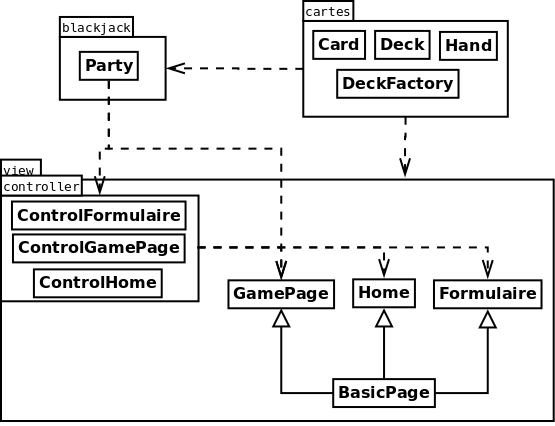
\includegraphics[scale=0.4]{img/jeu.png}	
\end{center}

\section{Eléments techiniques} \label{elemtech}

\subsection{Paquetages utilisées}

Dans le package \textsl{/lib} se trouve les paquetages JAR nécessaires au lancement du jeu:

\begin{table}[h]
	\begin{center}
		\begin{tabular}{| c | c |}
			\hline
			\textbf{nom librairie} & \textbf{utilité} \\
			\hline
  			cartes.jar & gestion jeu de cartes \\
 			\hline
  			hamcrest-2.2.jar & modules projectAPI \\
  			\hline
  			junit-4.13.2.jar & tests java \\
  			\hline
  			org-netbeans-modules-java-j2seproject-copylibstask.jar & tests\\
  			\hline
  			test.jar & nos tests \\
  			\hline
 		\end{tabular}
		\caption{Liste des archives .jar utilisées}
	\end{center}
\end{table}

\subsection{Pattern}

La classe \textsl{DeckFactory} est un pattern de construction. Elle génère des \textsl{Deck} prédéfinis de 52 ou 40 cartes.\\
Dans la classe \textsl{Party} du package \textsl{blackjack}, nous avons définit un pattern de strategy. En effet, cette classe contient la main du croupier, et les mains des IA, qui joue leur tour, une fois celui de l'utilisateur terminé.


\section{Conclusion} \label{conclusion}

Nous avons donc un jeu complet avec intelligences artificielles et patterns, c'était bien l'objectif que nous nous étions fixés. Nous n'avons malheureusement pas eu le temps d'implémenter plus de patterns mais nous sommes quand même fier de ce que nous avons produit.

\end{document}